So far, the applications of the structures we have discussed are primarily useful at compile- or design-time.
In this section we will discuss \acs{TETRiS}, a hybrid mapping approach where the structure of mapping symmetries are useful at run-time.

In Section~\ref{sec:symmetries} we saw how the symmetries of the mapping problem define multiple mappings to be equivalent.
We expect mappings that are equivalent to have the same runtime or energy consumption. Indeed, the simulation results are identical for equivalent mappings.
When leveraging this structure for \ac{DSE}, we consider only one of the multiple equivalent mappings, disregarding the rest, since they yield identical results in a simulation.
The \acf{TETRiS} approach~\cite{goens_scopes17} leverages this property in a complementary fashion, by selecting equivalent variants at run-time according to the current system load.
While this works for a single mapping, the strength of \ac{TETRiS} lies in selecting from different mappings with different properties first and using the equivalent variants to find a multi-application schedule.

\begin{figure*}[th]
	\centering
	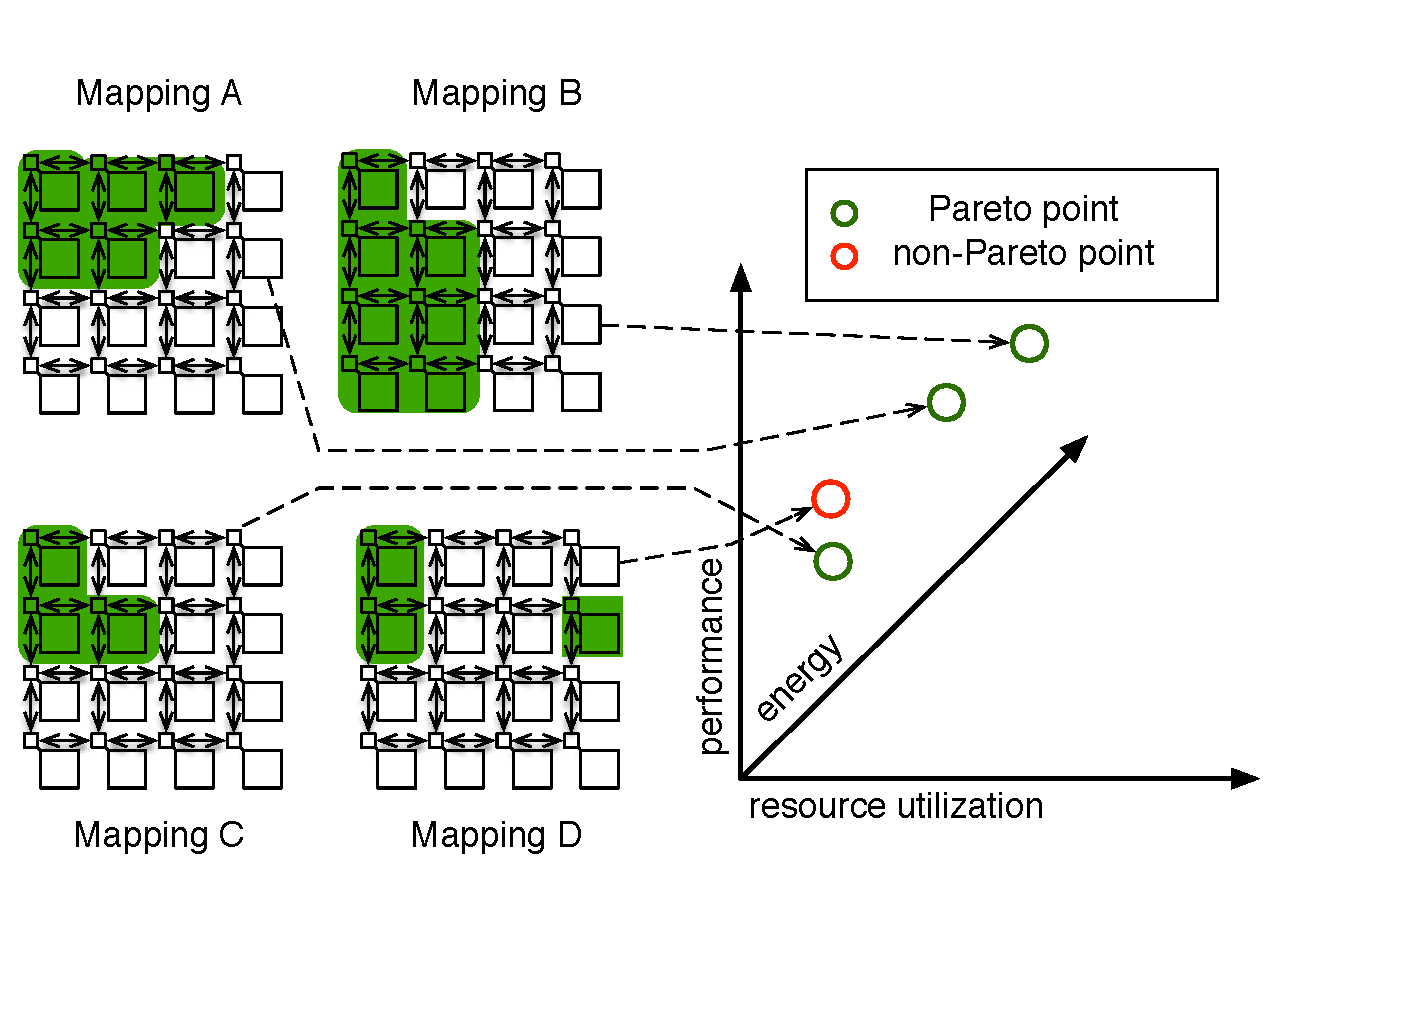
\includegraphics[width=0.7\textwidth]{figures/pareto_mappings.pdf}
	\caption{An illustration of Pareto points in the mapping space.}
	\label{fig:tetris_pareto}
\end{figure*}

We say that a design point (mapping) $m_1$ \emph{dominates} another $m_2$ if for the objective property $\Theta$, $m_1$ is at least as good as $m_2$: $\Theta(m_1) \leq \Theta(m_2)$. \index{dominated}
Recall that as defined in Equation~\ref{eqn:mapping_min_problem}, $\Theta$ is a multi-objective function and the comparison $\Theta(m_1) \leq \Theta(m_2)$ is to be understood component-wise, i.e. for each objective $i$, $\Theta_i(m_1) \leq \Theta_i(m_2)$.
A Pareto point is a design point (mapping), which is not dominated by any other design points. 
The different mappings \ac{TETRiS} chooses from are, ideally, Pareto points in the space of properties we are interested in.\index{Pareto point}
Figure~\ref{fig:tetris_pareto} illustrates this for the properties of energy, performance and resource utilization.
Each of the green points in the property space depicted to the right of the figure is a Pareto point.
It is better than every other point in at least one of the properties (performance, energy or resource utilization).
Only the red point corresponding to Mapping D is dominated by Mapping C, which utilizes the same number of resources, while being faster and more energy efficient.

The selection algorithms based on the desired properties are beyond the scope of this thesis, but \mocasin has implementations of multiple such algorithms~\cite{khasanov_date20}.
Once a mapping has been selected for each application, they need to be combined in a multi-application mapping.
This is where the symmetries come into play. 

\begin{figure*}[th]
	\centering
	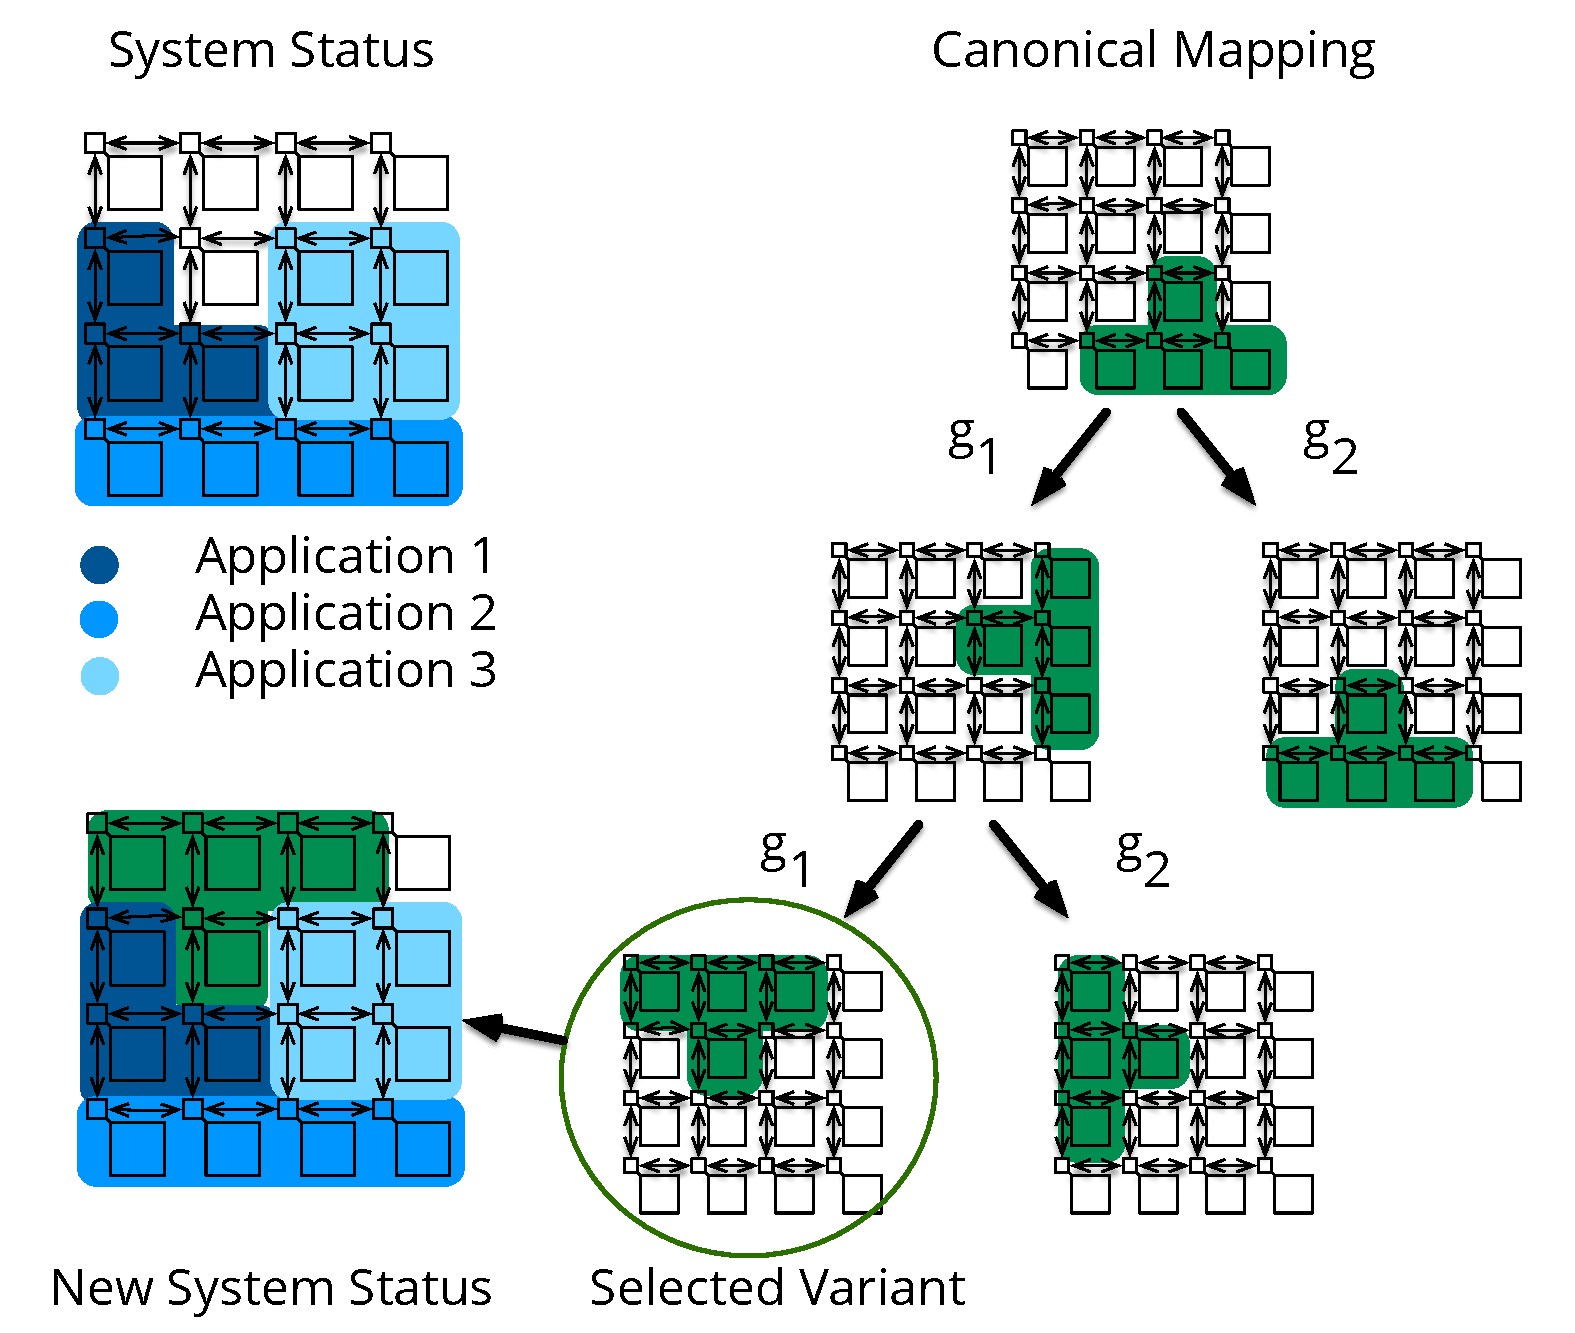
\includegraphics[width=0.8\textwidth]{figures/Variant_Selection.pdf}
	\caption{Variant selection in \ac{TETRiS}.}
	\label{fig:tetris_variant_selection}
\end{figure*}

Figure~\ref{fig:tetris_variant_selection} depicts the principle behind this symmetry-enabled variant selection.
At this point we assume a mapping has been selected, which we call the \emph{canonical mapping} in reference to the canonical representative of the equivalence class (orbit).\index{\ac{TETRiS} ! canonical mapping}
\ac{TETRiS} keeps track of the system's status, knowing where other running applications are mapped.
The idea behind the variant selection is then to apply the generators $g_i \in G$ of the automorphism group $G$ for the mapping space. 
We call the process of applying these generators \emph{\ac{TETRiS} rotations}, informed by the geometric intuition of these transformations\index{\ac{TETRiS} ! rotations}\footnote{This might be reminiscent of the commercial game Tetris. Note that the \ac{TETRiS} system is an independent research project and any resemblance is purely coincidental.}

\begin{figure*}[th]
	\centering
	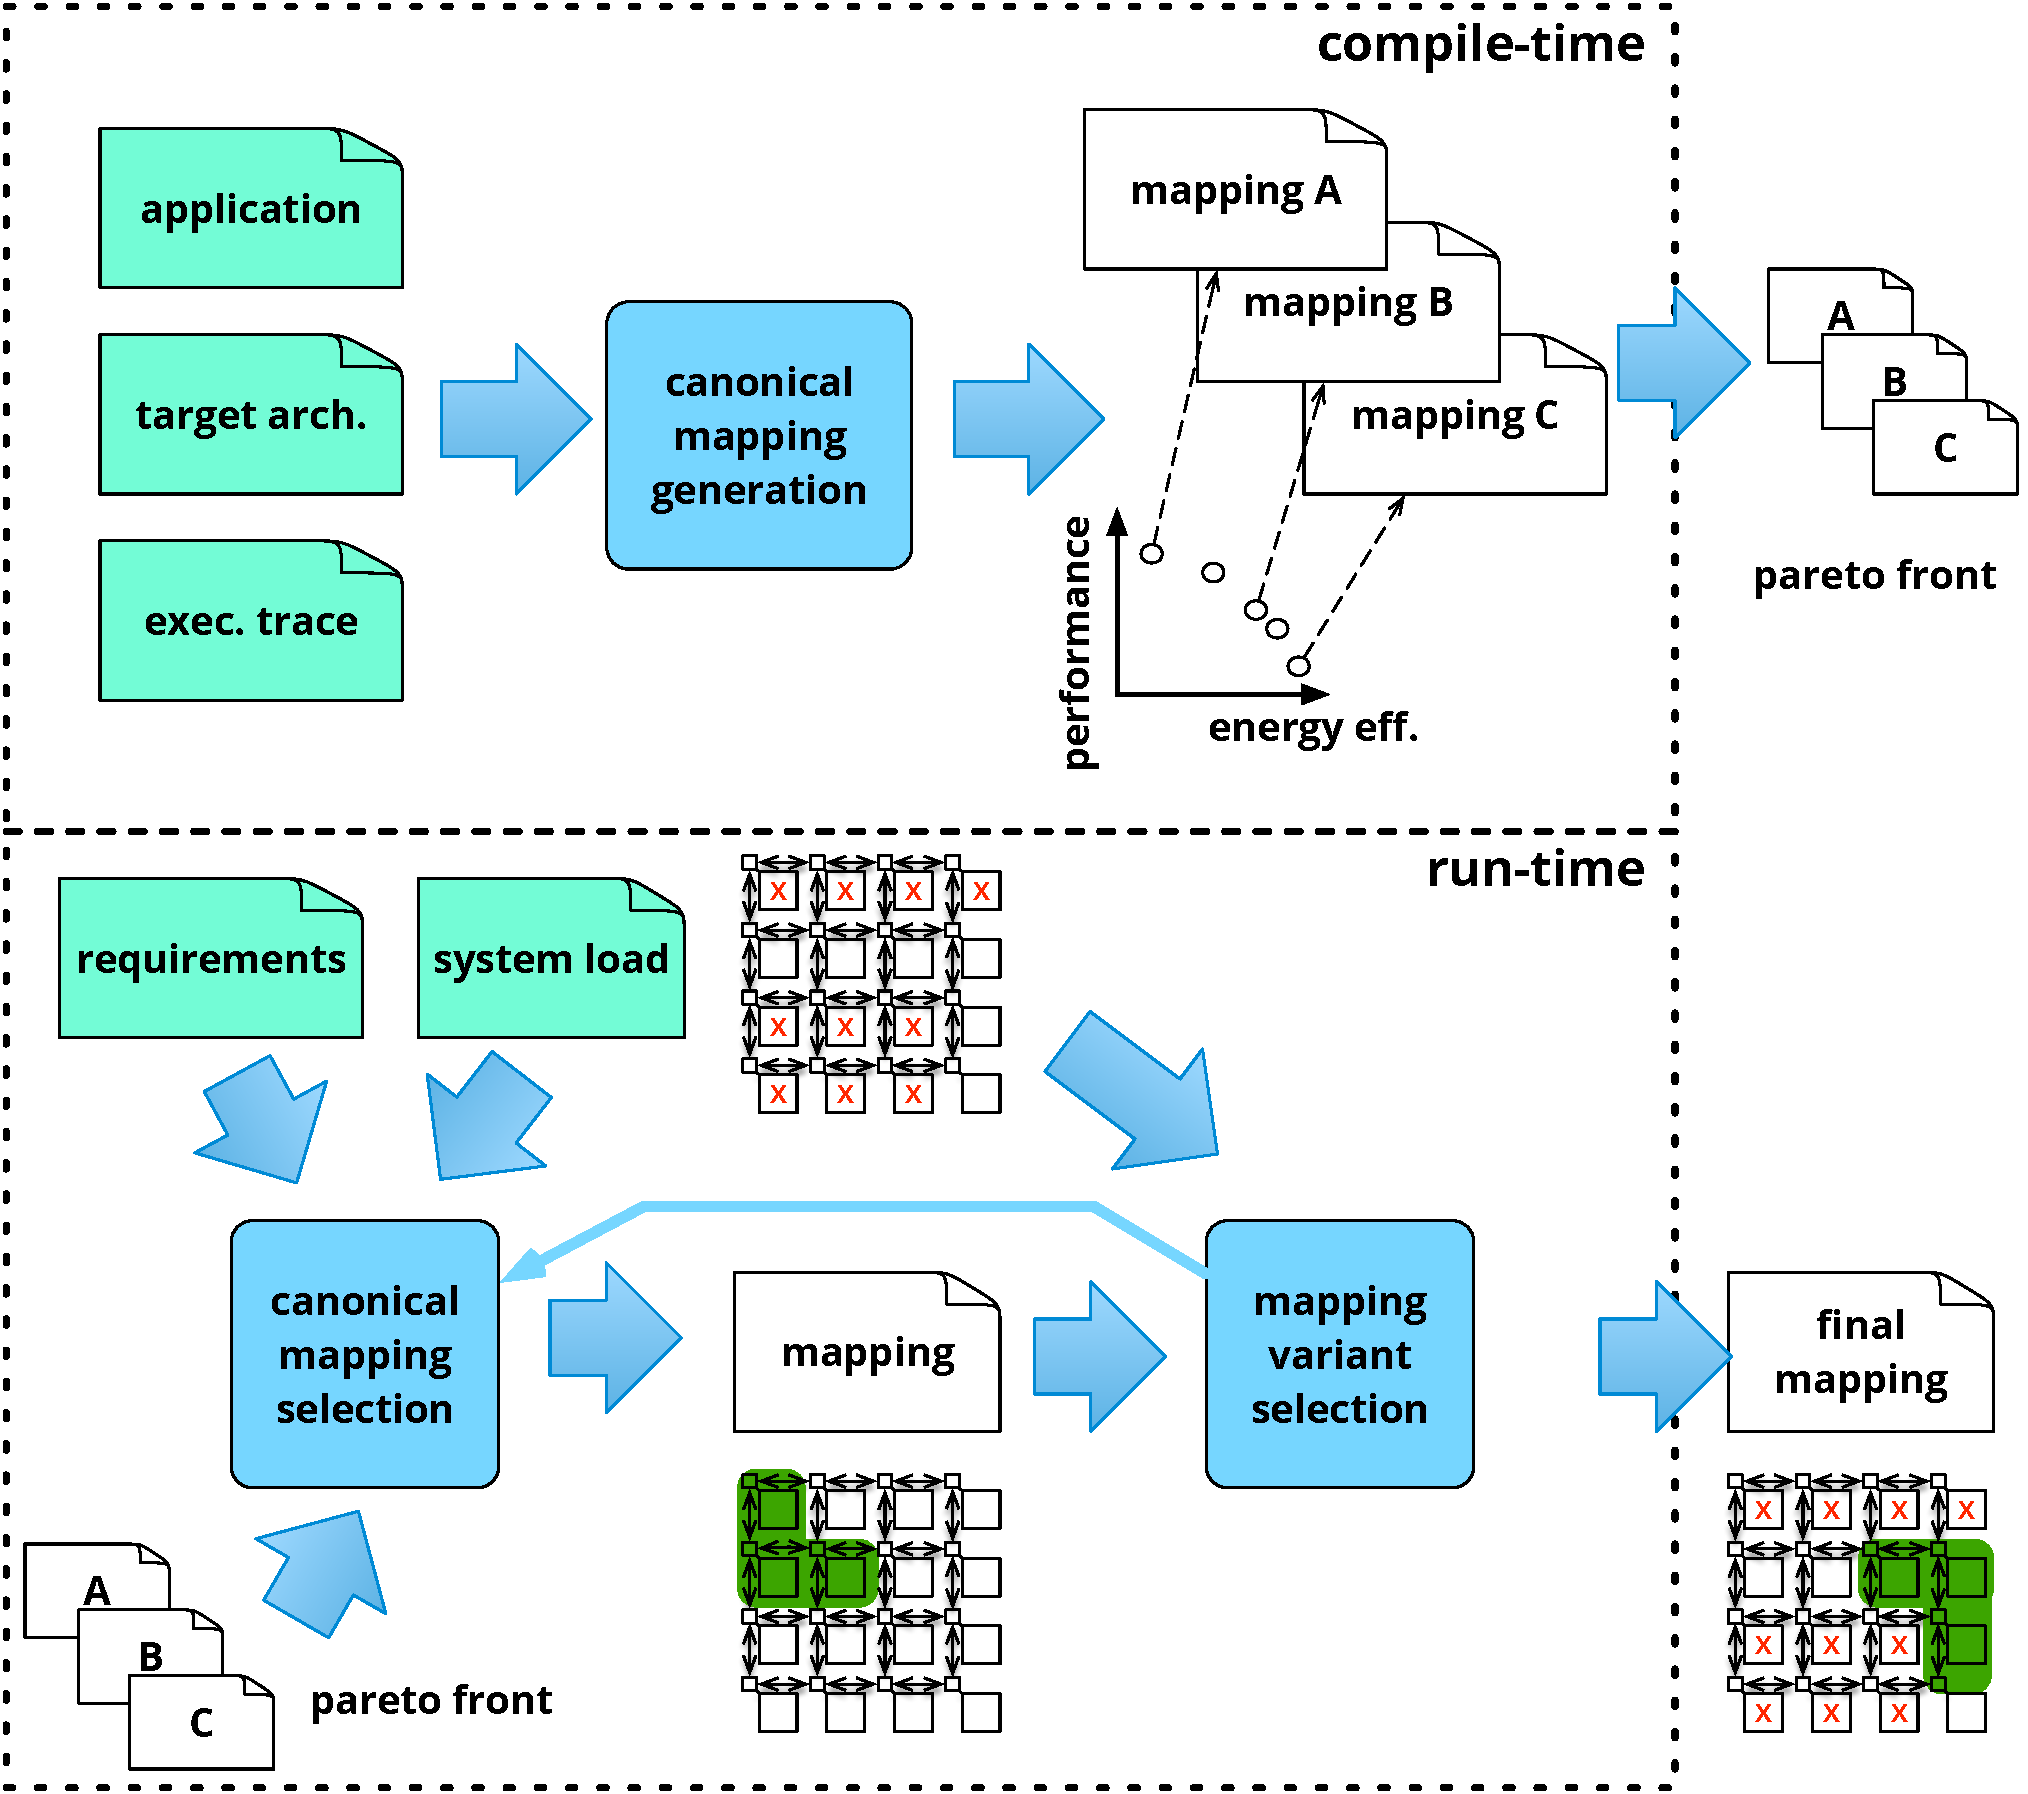
\includegraphics[width=1.00\textwidth]{figures/tetris_flow.pdf}
	\caption{The \ac{TETRiS} flow.}
	\label{fig:tetris_flow}
\end{figure*}

Combining the principles outlined above, Figure~\ref{fig:tetris_flow} shows the general flow of the hybrid \ac{TETRiS} approach. 
In a compile-time phase, so-called \ac{TETRiS} canonical mappings are generated as Pareto points in a multi-objective design space which ideally includes the system's resources as an objective.
Then, at run-time, a selection algorithm decides which canonical mapping to use based on the requirements (e.g. real-time constraints) and possibly also based on the system's load.
The selected canonical mapping is then placed onto the system by leveraging the symmetries of the mapping space in a variant selection phase, generating a final run-time mapping.
When generating mappings with this method, we can guarantee the spatial isolation of computation.
Provided the contention in communication is not too large, this also means that the properties of the canonical mappings are preserved (cf. Section~\ref{sec:compact}).
We tested this on an Odroid XU4 system running a pthread-based implementation\footnote{\url{https://github.com/l3nkz/tetris}} of the \ac{TETRiS} principle~\cite{goens_scopes17}.

\begin{figure*}[th]
	\centering
   \resizebox{0.95\textwidth}{!}{\inputTikz{tetris_experiment.tex}}
	\caption{Comparison of the TETRiS system with Linux' \acs*{CFS} executing four instances of the audio filter benchmark simultaneously an Odroid XU4. Adapted from Figure~9 in~\cite{goens_scopes17}.}
	\label{fig:tetris_experiment}
\end{figure*}

Figure~\ref{fig:tetris_experiment} shows the results of this test.
It compares the Linux \ac{CFS} with our \ac{TETRiS} system when running for instances of the audio filter benchmark (\ac{CPN}).
The three mappings $T_1$, $T_2$ and $T_3$ are three different Pareto points in terms of wall-clock time, CPU time and energy consumption. 
The mapping \ac{CFS} refers to an execution using Linux' \ac{CFS} scheduler and thus technically without a (static) mapping, which we measured for comparison.
For each mapping we executed the four concurrent instances of the application and measured the wall-clock and execution times as well as the total energy consumption.
We see that the execution of applications with \ac{TETRiS} is indeed significantly more predictable than with the dynamic approach of \ac{CFS}.
This is especially clear for the execution times, where the variance of \ac{CFS} of around $1.3 \cdot 10^{-1} s$ is two orders of magnitude higher than that of \ac{TETRiS}, which for example for $T_3$ is only  $2.7 \cdot 10^{-3}s$.
However, the difference is also very clearly visible for the energy consumption. The variance of \ac{CFS} is around $2.9 J$, whereas that of \ac{TETRiS} for $T_3$ is around $6.9 \cdot 10^{-1} J$, about an order of magnitude lower.

We have already implemented the symmetries and some of the algorithms of~\cite{khasanov_date20} in \mocasin.
 In future work we want to integrate the whole flow as depicted in Figure~\ref{fig:tetris_flow} for this.
In~\cite{menard_rapido21} we showed in preliminary results how this could yield an improvement over static mapping approaches.
There we evaluated the methods on a 5G use-case. This use-case will be discussed further in Section~\ref{sec:5g}.
Another avenue for future work is supporting OpenMP applications.
